\section{TensorFlow}
\label{chap:TensorFlow}

  %%%%%%%%%%%%%%%%%%%%%%%%%%%%
  % SUBSECTION               %
  %%%%%%%%%%%%%%%%%%%%%%%%%%%%
  \subsection{Introduction}
    The Google Brain project started in 2011 to explore the use of very-large-scale deep neural networks, both for research and for use in Google’s products. As part of the early work in this project, they built DistBelief, their first-generation scalable distributed training and inference system, and this system has served them well. They and others at Google have performed a wide variety of research using DistBelief including work on unsupervised learning, language representation, models for image classification and object detection, video classification, speech recognition, sequence prediction, move selection for Go, pedestrian detection, reinforcement learning, and other areas. In addition, often in close collaboration with the Google Brain team, more than 50 teams at Google and other Alphabet companies have deployed deep neural networks using DistBelief in a wide variety of products, including Google Search, Their advertising products, speech recognition systems, Google Photos, Google Maps and StreetView, Google Translate, YouTube, and many others.\cite{tensorflow2015-whitepaper}\\
    Based on their experience with DistBelief and a more complete understanding of the desirable system properties and requirements for training and using neural networks, they have built TensorFlow, their second-generation system for the implementation and deployment of largescale machine learning models. TensorFlow takes computations described using a dataflow-like model and maps them onto a wide variety of different hardware platforms, ranging from running inference on mobile device platforms such as Android and iOS to modestsized training and inference systems using single machines containing one or many GPU cards to large-scale training systems running on hundreds of specialized machines with thousands of GPUs. Having a single system that can span such a broad range of platforms significantly simplifies the real-world use of machine learning system, as they have found that having separate systems for large-scale training and small-scale deployment leads to significant maintenance burdens and leaky abstractions.\cite{tensorflow2015-whitepaper}\\
    TensorFlow is an interface for expressing machine learning algorithms, and an implementation for executing such algorithms. A computation expressed using TensorFlow can be executed with little or no change on a wide variety of heterogeneous systems, ranging from mobile devices such as phones and tablets up to large-scale distributed systems of hundreds of machines and thousands of computational devices such as GPU cards. The system is flexible and can be used to express a wide variety of algorithms, including training and inference algorithms for deep neural network models, and it has been used for conducting research and for deploying machine learning systems into production across more than a dozen areas of computer science and other fields, including speech recognition, computer vision, robotics, information retrieval, natural language processing, geographic information extraction, and computational drug discovery.\cite{tensorflow2015-whitepaper}\\
    TensorFlow is an open-source software library for dataflow programming across a range of tasks, and is arguably one of the best deep learning frameworks and has been adopted by several giants such as Airbus, Twitter, IBM, and others mainly due to its highly flexible system architecture. It is available on both desktop and mobile and also supports languages such as Python, C++, and R to create deep learning models along with wrapper libraries.\cite{web021}
    \subsubsection{CUDA and TensorFlow}
    CUDA or Compute Unified Device Architecture is an API for Parallel Computing by NVIDIA. CUDA allows you to harness the power of your GPU for computing applications. They (GPUs) can do parallel processing much faster/better than traditional chips (CPUs).\\
    Now, if you've gone through the install docs for Tensorflow using NVIDIA GPUs, you will notice they ask you to install CUDA libraries and toolkits first. It is only then, that Tensorflow can harness the power and speed of computation that your GPU would offer you.\\
    Tensorflow will access the better computation power of NVIDIA GPUs via (or using, both terms are interchangeable here) the CUDA API.\\
    You can absolutely perform tensorflow’s computations from GPUs, but in case you're using an NVIDIA GPU, you need to have CUDA installed so that Tensorflow can actually access what that awesome NVIDIA GPU has to offer with all its parallel computing capable, CUDA Cores.
    \subsection{Tensors}
    TensorFlow, as the name indicates, is a framework to define and run computations involving tensors. A tensor is a generalization of vectors and matrices to potentially higher dimensions. Internally, TensorFlow represents tensors as n-dimensional arrays of base datatypes.\\
    When writing a TensorFlow program, the main object you manipulate and pass around is the. A \textbf{tf.Tensor} object represents a partially defined computation that will eventually produce a value. TensorFlow programs work by first building a graph of \textbf{tf.Tensor} objects, detailing how each tensor is computed based on the other available tensors and then by running parts of this graph to achieve the desired results.\cite{web022}\\
    A \textbf{tf.Tensor} has the following properties:
    \begin{enumerate}
      \item\textbf{a data type}\\ 
      (float32, int32, or string, for example)
      \item\textbf{a shape}
      \end{enumerate}
      Each element in the Tensor has the same data type, and the data type is always known. The shape (that is, the number of dimensions it has and the size of each dimension) might be only partially known. Most operations produce tensors of fully-known shapes if the shapes of their inputs are also fully known, but in some cases it's only possible to find the shape of a tensor at graph execution time.
    \subsubsection{Types of tensors}
      \begin{enumerate}
    \item\textbf{tf.Variable}
    \item\textbf{tf.constant}
    \item\textbf{tf.placeholder}
    \end{enumerate}
    \paragraph{Variables}
    A variable maintains state in the graph across calls to run(). You add a variable to the graph by constructing an instance of the class Variable.
    The Variable() constructor requires an initial value for the variable, which can be a Tensor of any type and shape. The initial value defines the type and shape of the variable. After construction, the type and shape of the variable are fixed. The value can be changed using one of the assign methods.
    If you want to change the shape of a variable later you have to use an assign Op with validate-shape=False.
    Just like any Tensor, variables created with Variable() can be used as inputs for other Ops in the graph. Additionally, all the operators overloaded for the Tensor class are carried over to variables, so you can also add nodes to the graph by just doing arithmetic on variables.
    \begin{lstlisting}[language=Python]
import tensorflow as tf
# Create a variable.
w = tf.Variable(<initial-value>, name=<optional-name>)
# Use the variable in the graph like any Tensor.
y = tf.matmul(w, ...another variable or tensor...)
# The overloaded operators are available too.
z = tf.sigmoid(w + y)
# Assign a new value to the variable with `assign()` or a related method.
w.assign(w + 1.0)
w.assign_add(1.0)
\end{lstlisting}
\paragraph{Constants}
Creates a constant tensor.
The resulting tensor is populated with values of type dtype, as specified by arguments value and (optionally) shape .
The argument value can be a constant value, or a list of values of type dtype. If value is a list, then the length of the list must be less than or equal to the number of elements implied by the shape argument (if specified). In the case where the list length is less than the number of elements specified by shape, the last element in the list will be used to fill the remaining entries.
The argument shape is optional. If present, it specifies the dimensions of the resulting tensor. If not present, the shape of value is used.
If the argument dtype is not specified, then the type is inferred from the type of value.
\begin{lstlisting}[language=Python]
# Constant 1-D Tensor populated with value list.
tensor = tf.constant([1, 2, 3, 4, 5, 6, 7]) => [1 2 3 4 5 6 7]
# Constant 2-D tensor populated with scalar value -1.
tensor = tf.constant(-1.0, shape=[2, 3]) => [[-1. -1. -1.]
                                             [-1. -1. -1.]]

\end{lstlisting}
\paragraph{Placeholder}
So far we have used Variables to manage our data, but there is a more basic structure, the placeholder. A placeholder is simply a variable that we will assign data to at a later date. It allows us to create our operations and build our computation graph, without needing the data. In TensorFlow terminology, we then feed data into the graph through these placeholders.
This tensor will produce an error if evaluated. Its value must be fed using the \textbf{feed-dict} optional argument to \textbf{Session.run()}, \textbf{Tensor.eval()}, or \textbf{Operation.run()}.
\begin{lstlisting}[language=Python]
x = tf.placeholder(tf.float32, shape=(1024, 1024))
y = tf.matmul(x, x)
with tf.Session() as sess:
  print(sess.run(y))  # ERROR: will fail because x was not fed.
  rand_array = np.random.rand(1024, 1024)
  print(sess.run(y, feed_dict={x: rand_array}))  # Will succeed.
\end{lstlisting}
    \subsubsection{TensorFlow operations}
    
    \begin{table}[H] \centering  

\begin{tabular}{ |p{7cm}||p{9cm} |p{3cm}|p{3cm}| }
 \hline
 \multicolumn{2}{|c|}{Operations} \\
 \hline
 
 Category & Examples \\
 \hline
 Mathematical operations & Add, Sub, Mul, Div, Exp, Log,...\\
 Array operations & Concat, Slice, Split, Constant, Rank, Shape,...\\
 Matrix operations & MatMul, MatrixInverse, MatrixDeterminant,...\\
 Stateful operations & Variable, Assign, AssignAdd,...\\
 Neural Network building blocks & SoftMax, Sigmoid, ReLU, Convolution2D, MaxPool,...\\
 Checkpointing operations & Save, Reestore\\
 Queue and synchronization operations & Enqueue, Dequeue, MutexAcquire, MutexRelease,...\\
 Control flow operations & Merge, Switch, Enter, Leave, NextIteration\\
 
 
 \hline
 
\end{tabular}
\caption{Operations of Tensorflow \cite{web010}}
\label{table:1}

\end{table}

\subsection{Graphs and Sessions}
TensorFlow uses a dataflow graph to represent your computation in terms of the dependencies between individual operations. This leads to a low-level programming model in which you first define the dataflow graph, then create a TensorFlow session to run parts of the graph across a set of local and remote devices.\\
  \textbf{Why Dataflow Graphs?}\\
  Dataflow is a common programming model for parallel computing. In a dataflow graph, the nodes represent units of computation, and the edges represent the data consumed or produced by a computation.\\
  For example, in a TensorFlow graph, the \textbf{tf.matmul} operation would correspond to a single node with two incoming edges (the matrices to be multiplied) and one outgoing edge (the result of the multiplication).\\
Dataflow has several advantages that TensorFlow leverages when executing programs:
\begin{enumerate}
      \item\textbf{Parallelism.}
\item\textbf{Distributed execution.}
\item\textbf{Compilation.}
\item\textbf{Portability.}
\end{enumerate}
\begin{figure}[H]%
    \center%
    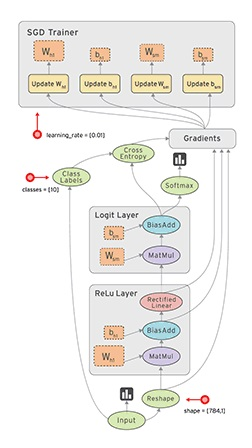
\includegraphics[width=0.5\textwidth]{images/eman/Dataflow-graph.jpg}%
     % you need to add the caption for the list of figures
\caption[This is Dataflow Graph]{Dataflow Graph}\label{fig:graph}%
  \end{figure}

\paragraph{Graphs}
A \textbf{tf.Graph} contains two relevant kinds of information:
\begin{enumerate}
      \item\textbf{Graph structure}\\
      The nodes and edges of the graph, indicating how individual operations are composed together, but not prescribing how they should be used. The graph structure is like assembly code: inspecting it can convey some useful information, but it does not contain all of the useful context that source code conveys.
      
      \item\textbf{Graph collections}\\
      TensorFlow provides a general mechanism for storing collections of metadata in a \textbf{tf.Graph.} The \textbf{tf.add-to-collection} function enables you to associate a list of objects with a key (where \textbf{tf.GraphKeys} defines some of the standard keys), and \textbf{tf.get-collection} enables you to look up all objects associated with a key. Many parts of the TensorFlow library use this facility: for example, when you create a \textbf{tf.Variable}, it is added by default to collections representing "global variables" and "trainable variables". When you later come to create a \textbf{tf.train.Saver} or \textbf{tf.train.Optimizer}, the variables in these collections are used as the default arguments.
      
\end{enumerate}

\paragraph{Sessions}
    TensorFlow uses the \textbf{tf.Session} class to represent a connection between the client program ---typically a Python program, although a similar interface is available in other languages--- and the C++ runtime. A \textbf{tf.Session} object provides access to devices in the local machine, and remote devices using the distributed TensorFlow runtime. It also caches information about your \textbf{tf.Graph} so that you can efficiently run the same computation multiple times.\\
    \begin{lstlisting}[language=Python]
# Create a default in-process session.
with tf.Session() as sess:
  # ...
# Create a remote session.
with tf.Session("grpc://example.org:2222"):
  # ...

\end{lstlisting}

    Since a \textbf{tf.Session} owns physical resources (such as GPUs and network connections), it is typically used as a context manager (in a with block) that automatically closes the session when you exit the block. It is also possible to create a session without using a with block, but you should explicitly call \textbf{tf.Session.close} when you are finished with it to free the resources.\\
    \textbf{Note: }In Tensorflow you have an execution graph, which takes inputs and produces outputs. Naturally you \textbf{feed} the inputs into the graph, run it, and then \textbf{fetch} the outputs back into your program.
    \subsection{Save and restore models}
    \subsubsection{Meta graph}
    This is a protocol buffer which saves the complete Tensorflow graph; i.e. all variables, operations, collections etc. This file has .meta extension.
    \subsubsection{Checkpoints}
    TensorFlow provides two model formats:
    \begin{enumerate}
      \item\textbf{checkpoints}\\
      which is a format dependent on the code that created the model.
    \item\textbf{SavedModel}\\ 
    which is a format independent of the code that created the model.
    \end{enumerate}
Here, we will focus on checkpoints.\\
\textbf{Saving partially-trained models}\\
Estimators automatically write the following to disk:
\begin{enumerate}
      \item\textbf{checkpoints}\\
      which are versions of the model created during training.
      \item\textbf{event files}\\
      which contain information that TensorBoard uses to create visualizations.
      \end{enumerate}
      To specify the top-level directory in which the Estimator stores its information, assign a value to the optional model-dir argument of any Estimator's constructor. For example, the following code sets the model-dir argument to the models/iris directory:
      \begin{lstlisting}[language=Python]
classifier = tf.estimator.DNNClassifier(
    feature_columns=my_feature_columns,
    hidden_units=[10, 10],
    n_classes=3,
    model_dir='models/iris')

\end{lstlisting}
Suppose you call the Estimator's train method. For example:
\begin{lstlisting}[language=Python]
cclassifier.train(
        input_fn=lambda:train_input_fn(train_x, train_y, batch_size=100),
                steps=200)

\end{lstlisting}
As suggested by the following diagrams, the first call to train adds checkpoints and other files to the model-dir directory:
\begin{figure}[H]%
    \center%
    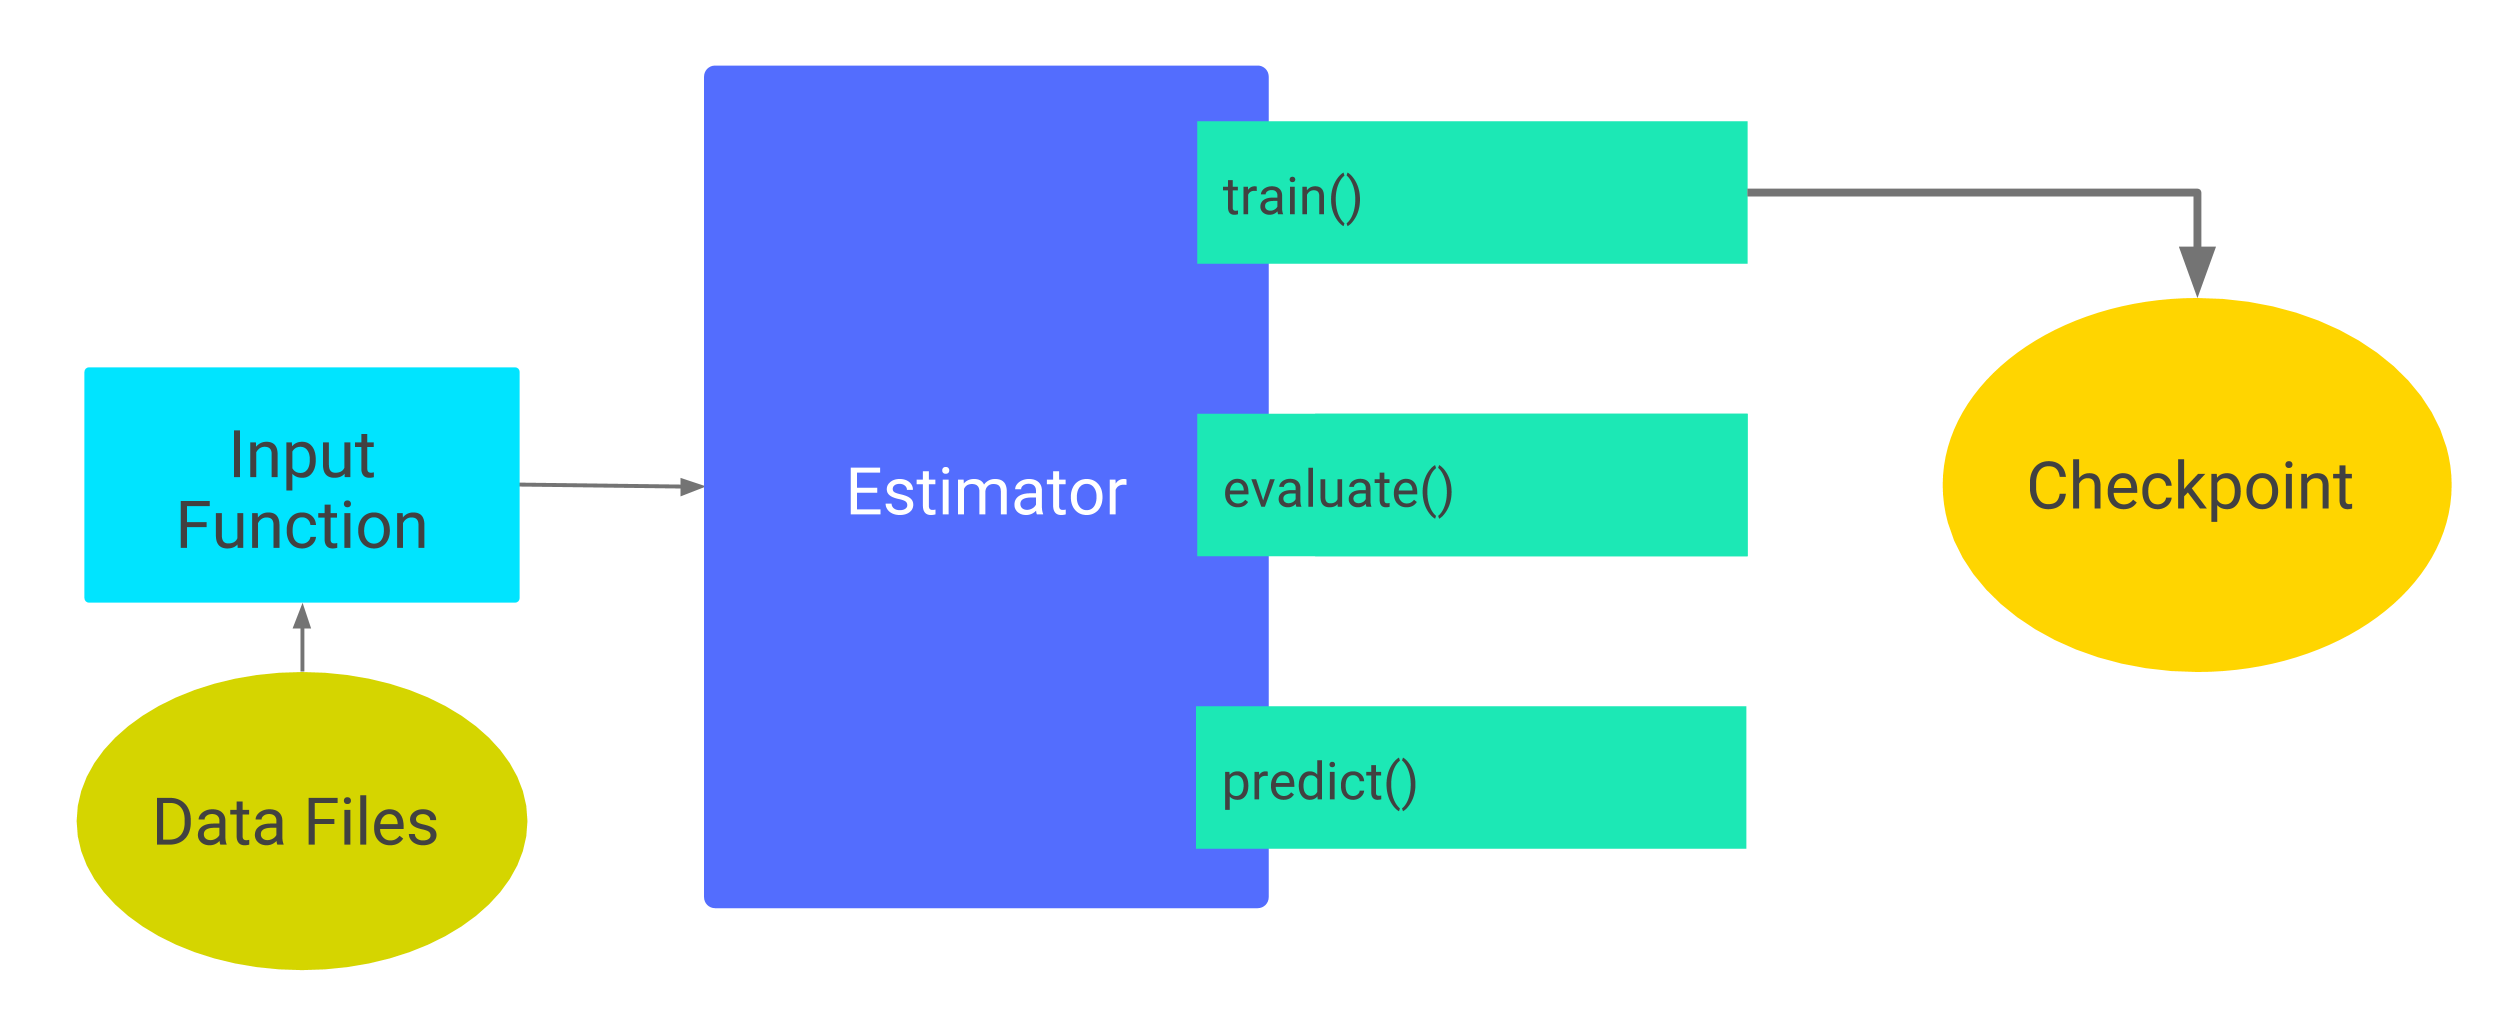
\includegraphics[width=0.8\textwidth]{images/eman/first_train_calls.png}%
     % you need to add the caption for the list of figures
\caption[This is first train call]{The first call to train()}\label{fig:call}%
  \end{figure}
  
  \subsection{Training}
  \textbf{tf.train} provides a set of classes and functions that help train models.
  \subsubsection{Optimizers}
  The Optimizer base class provides methods to compute gradients for a loss and apply gradients to variables. A collection of subclasses implement classic optimization algorithms such as GradientDescent and Adagrad.\\
You never instantiate the Optimizer class itself, but instead instantiate one of the subclasses.
\begin{enumerate}
      \item\textbf{tf.train.Optimizer}\\
      This class defines the API to add Ops to train a model. We never use this class directly, but instead instantiate one of its subclasses such as GradientDescentOptimizer, AdagradOptimizer, or MomentumOptimizer.
      \item\textbf{tf.train.GradientDescentOptimizer}\\
      Optimizer that implements the gradient descent algorithm.
      \item\textbf{tf.train.AdadeltaOptimizer}\\
      Optimizer that implements the Adadelta algorithm.\cite{DBLP:journals/corr/abs-1212-5701}
      \item\textbf{tf.train.AdadeltaOptimizer}\\
      Optimizer that implements the Adagrad algorithm.\cite{Duchi:2011:ASM:1953048.2021068}
      \item\textbf{tf.train.AdagradDAOptimizer}\\
      Adagrad Dual Averaging algorithm for sparse linear models.
This optimizer takes care of regularization of unseen features in a mini batch by updating them when they are seen with a closed form update rule that is equivalent to having updated them on every mini-batch.
AdagradDA is typically used when there is a need for large sparsity in the trained model. This optimizer only guarantees sparsity for linear models. Be careful when using AdagradDA for deep networks as it will require careful initialization of the gradient accumulators for it to train.\cite{Duchi:2011:ASM:1953048.2021068}
      \item\textbf{tf.train.MomentumOptimizer}\\
      Optimizer that implements the Momentum algorithm.
      \item\textbf{tf.train.AdamOptimizer}\\
      Optimizer that implements the Adam algorithm.\cite{DBLP:journals/corr/KingmaB14}
      \item\textbf{tf.train.FtrlOptimizer}\\
      Optimizer that implements the FTRL algorithm.\cite{41159}
      \item\textbf{tf.train.ProximalGradientDescentOptimizer}\\
      Optimizer that implements the proximal gradient descent algorithm.\cite{NIPS2009_3793}
      \item\textbf{tf.train.ProximalAdagradOptimizer}\\
      Optimizer that implements the Proximal Adagrad algorithm.\cite{NIPS2009_3793}
      \item\textbf{tf.train.RMSPropOptimizer}\\
      Optimizer that implements the RMSProp algorithm.\cite{web027}
      \end{enumerate}
      \subsection{Backpropagation}
      Backpropagation is a method used in artificial neural networks to calculate a gradient that is needed in the calculation of the weights to be used in the network. It is commonly used to train deep neural networks, a term referring to neural networks with more than one hidden layer.
      \subsubsection{Motivation}
      The motivation for backpropagation is to train a multi-layered neural network such that it can learn the appropriate internal representations to allow it to learn any arbitrary mapping of input to output.
      \subsubsection{Loss function}
      Sometimes referred to as the cost function or error function (not to be confused with the Gauss error function), the loss function is a function that maps values of one or more variables onto a real number intuitively representing some "cost" associated with those values. For backpropagation, the loss function calculates the difference between the network output and its expected output, after a case propagates through the network.
      \subsubsection{Optimization}
      The optimization algorithm repeats a two phase cycle, propagation and weight update. When an input vector is presented to the network, it is propagated forward through the network, layer by layer, until it reaches the output layer. The output of the network is then compared to the desired output, using a loss function. The resulting error value is calculated for each of the neurons in the output layer. The error values are then propagated from the output back through the network, until each neuron has an associated error value that reflects its contribution to the original output.
Backpropagation uses these error values to calculate the gradient of the loss function. In the second phase, this gradient is fed to the optimization method, which in turn uses it to update the weights, in an attempt to minimize the loss function.
\subsubsection{Backpropagation with TensorFlow}
As we now know, TensorFlow from Google is an open source library that primarily focuses on deep learning. It uses computational data-flow graphs to represent complicated neural-network architecture. The nodes in the graph denote mathematical computations, also called ops (operations), whereas the edges denote the data tensors transferred between them.\\
Also, the relevant gradients are stored at each node of the computational graph, and during backpropagation these are combined to get the gradients with respect to each weight. Tensors are multi-dimensional data arrays used by TensorFlow.\\

\textbf{RMSprop:}\\
RMSprop is the mini-batch version of the resilient backpropagation (Rprop) optimization technique that works best for full-batch learning. Rprop solves the issue of gradients’ not pointing to the minimum in cases where the cost function contours are elliptical. In such cases, instead of a global learning rule a separate adaptive update rule for each weight would lead to better convergence. The special thing with Rprop is that it doesn’t use the magnitude of the gradients of the weight but only the signs in determining how to update each weight.\\


  



 
  


      
  


%%%%%%%%%%%%%%%%%%%%%%%%%%%%%%%%%%%%%%%%%%%%%%%%%%%%%%%%%%%%%%%%%%%%%%%%%%%%%%%%%%%%%%%%%%%%%%%%%%%%%%%%%%%%%%%%%%